\chapter{アプリケーション例}
\$Vを利用したアプリケーション例を本章にて示す.
\$Vは少ない学習データにおいて,高い認識率及び識別性能を示すため,ユーザ定義手書きジェスチャを利用したアプリケーションを開発することができる.
また,同じ形状及び書き順の手書きジェスチャを大きさ,向き,位置に関して識別可能であるため,それらを利用したアプリケーション例を示す.

\section{PCアプリケーション}
スマートフォンを手書きジェスチャの入力端末として用い,PC上のアプリケーションを操作可能な,PCとスマートフォンを連携したPCアプリケーションの例を示す.
\subsection{メディアプレイヤ}
図\ref{fig:application}のようなメディアプレイヤを開発することができる.
このメディアプレイヤにおいて,再生,巻き戻し,前のメディア,次のメディアなどに対し,同じ書き順及び同じ形状の手書きジェスチャが複数割り当てられており(図\ref{fig:application}a),それぞれ,大きさ,向き,位置の違いが利用されている.ユーザはスマートフォンを手書きジェスチャの入力端末として用いることによって,PC上のメディアプレイヤを操作することが可能である(図\ref{fig:application}b).

\begin{figure} [h!]
	\begin{center}
		\includegraphics [width=1.0\hsize ]{img/application.eps}
	\end{center}
	\caption{ツールキットを使って開発されたメディアプレイヤの例.(a)アプリケーションのスクリーンショット,(b)PC上のメディアプレイヤをスマートフォンを用いて操作している場面.}
	\label{fig:application}
\end{figure}

\subsubsection{開発ツールキット}
図\ref{fig:flow}に示すアプリケーション開発ツールキットは,本アプリケーションを開発するためのツールキットの例である.

まず,ユーザは,入力として用いたい手書きジェスチャを実際に手書きジェスチャを入力する端末を用いて学習データとして1つずつ追加していく(図\ref{fig:flow}a).
すると,\$Vが実装された本ツールキットは,追加された学習データを自動的にジェスチャグループに分類し,それぞれのジェスチャグループごとに,大きさ,向き,位置の特徴量に対する最適な重みを自動計算する(図\ref{fig:flow}b).
最後に,ユーザは,利用したいアプリケーションにおける処理を実行するAppleScriptあるいはボタンと利用したい手書きジェスチャを対応付けることによって(図\ref{fig:flow}c),手書きジェスチャを利用したアプリケーションを開発することができる.

\begin{figure} [h!]
	\begin{center}
		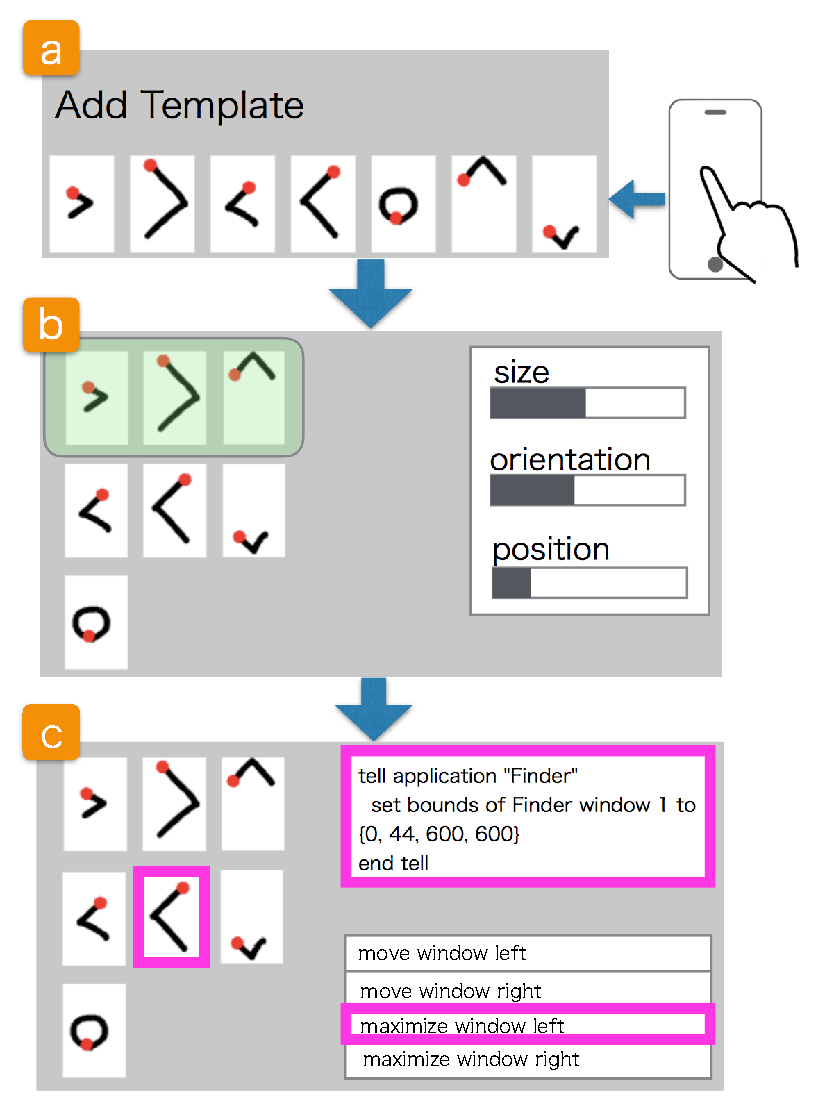
\includegraphics [width=0.7\hsize ]{img/flow.eps}
	\end{center}
	\caption{手書きジェスチャを利用したアプリケーション開発ツールキット.(a)まず,ユーザはスマートフォンなどの手書きジェスチャを入力する端末を用いて学習データを追加することによって,(b)\$Vが実装されたツールキットが,学習データを自動的にジェスチャグループに分類し,重みを計算する.(c)最後にユーザは,アプリケーションにおける処理と手書きジェスチャを対応付ける.}
	\label{fig:flow}
\end{figure}


\clearpage
\section{スマートフォンアプリケーション}
スマートフォンを手書きジェスチャの入力端末として用い,スマートフォン内のアプリケーションが操作可能なスマートフォンアプリケーションの例を示す.
\subsection{ブラウザ}
図\ref{fig:application}のようなブラウザを開発することができる.
このブラウザにおいて,同じ書き順及び同じ形状であるが,位置の違いを利用した手書きジェスチャが,ページの表示位置に対し割り当てられている(図\ref{fig:phone_web}).
また,手書きジェスチャが書かれた位置によってブックマークの登録先を決める,などのような動作を設定することができる(図\ref{fig:phone_bookmark}).

\begin{figure} [h!]
	\begin{center}
		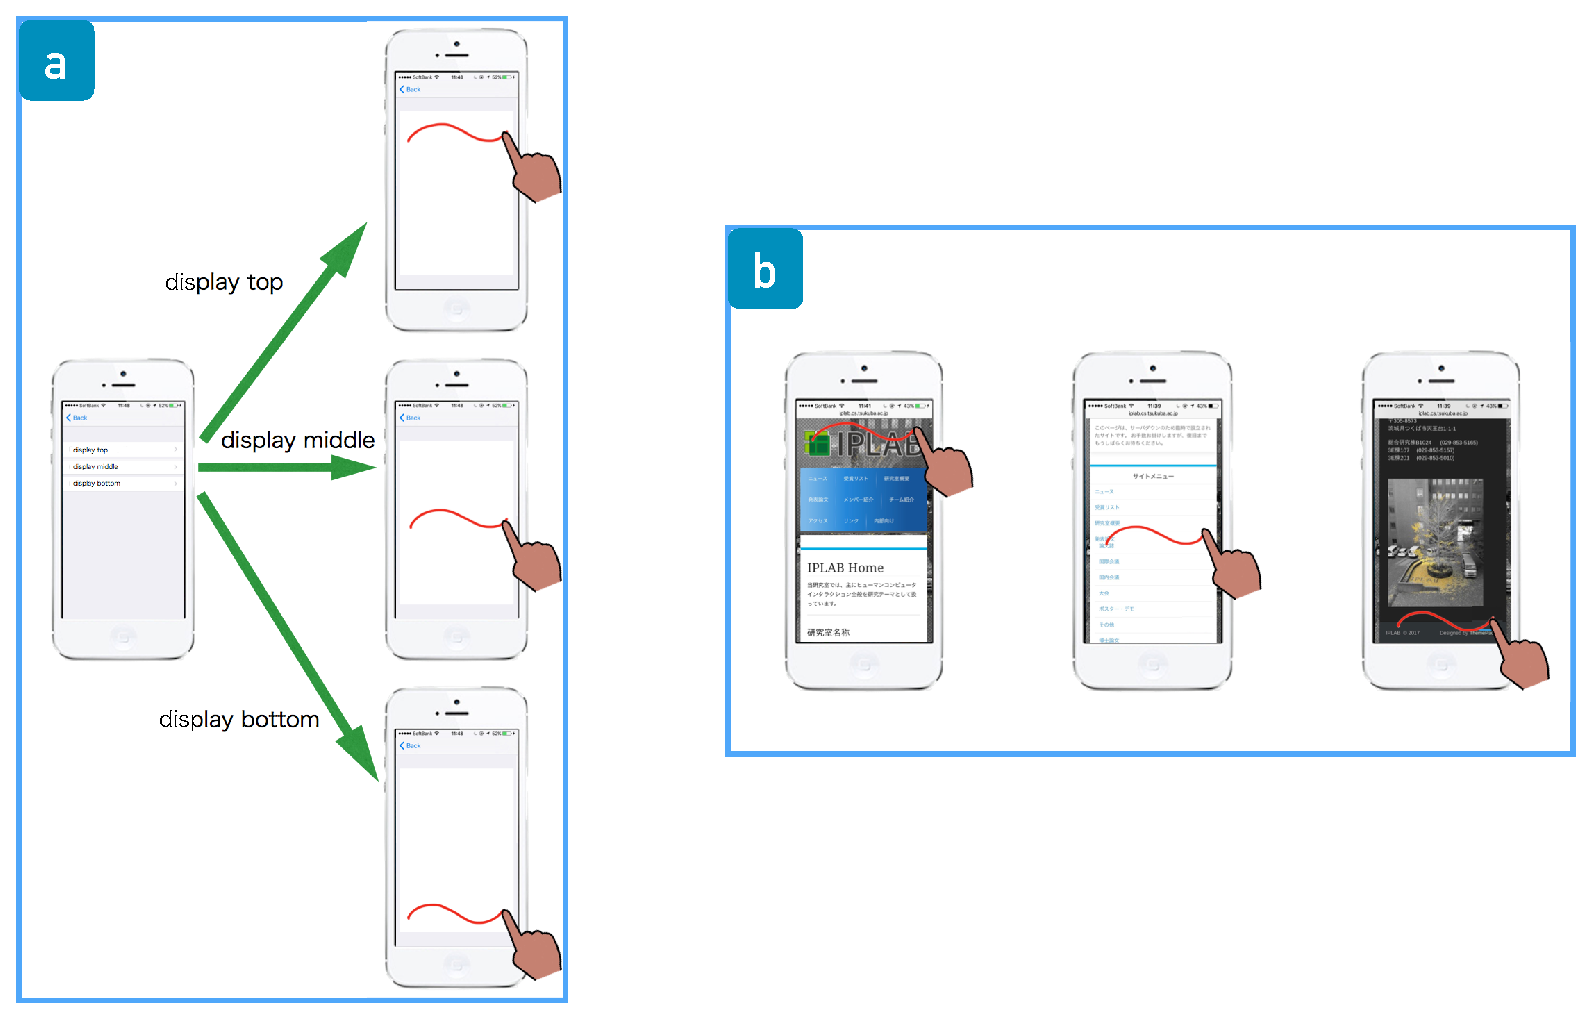
\includegraphics [width=1.0\hsize ]{img/phone_web.eps}
	\end{center}
	\caption{ブラウザにおいて,手書きジェスチャによりページの表示位置を指定している例.(a)同じ書き順及び同じ形状であるが,位置の違いをページの表示位置に割り当てる.(b)画面の上部に入力した場合ページ上部が,画面の中部に入力した場合ページ中部が,画面の下部に入力した場合ページ下部が表示される.}
	\label{fig:phone_web}
\end{figure}

\begin{figure} [h!]
	\begin{center}
		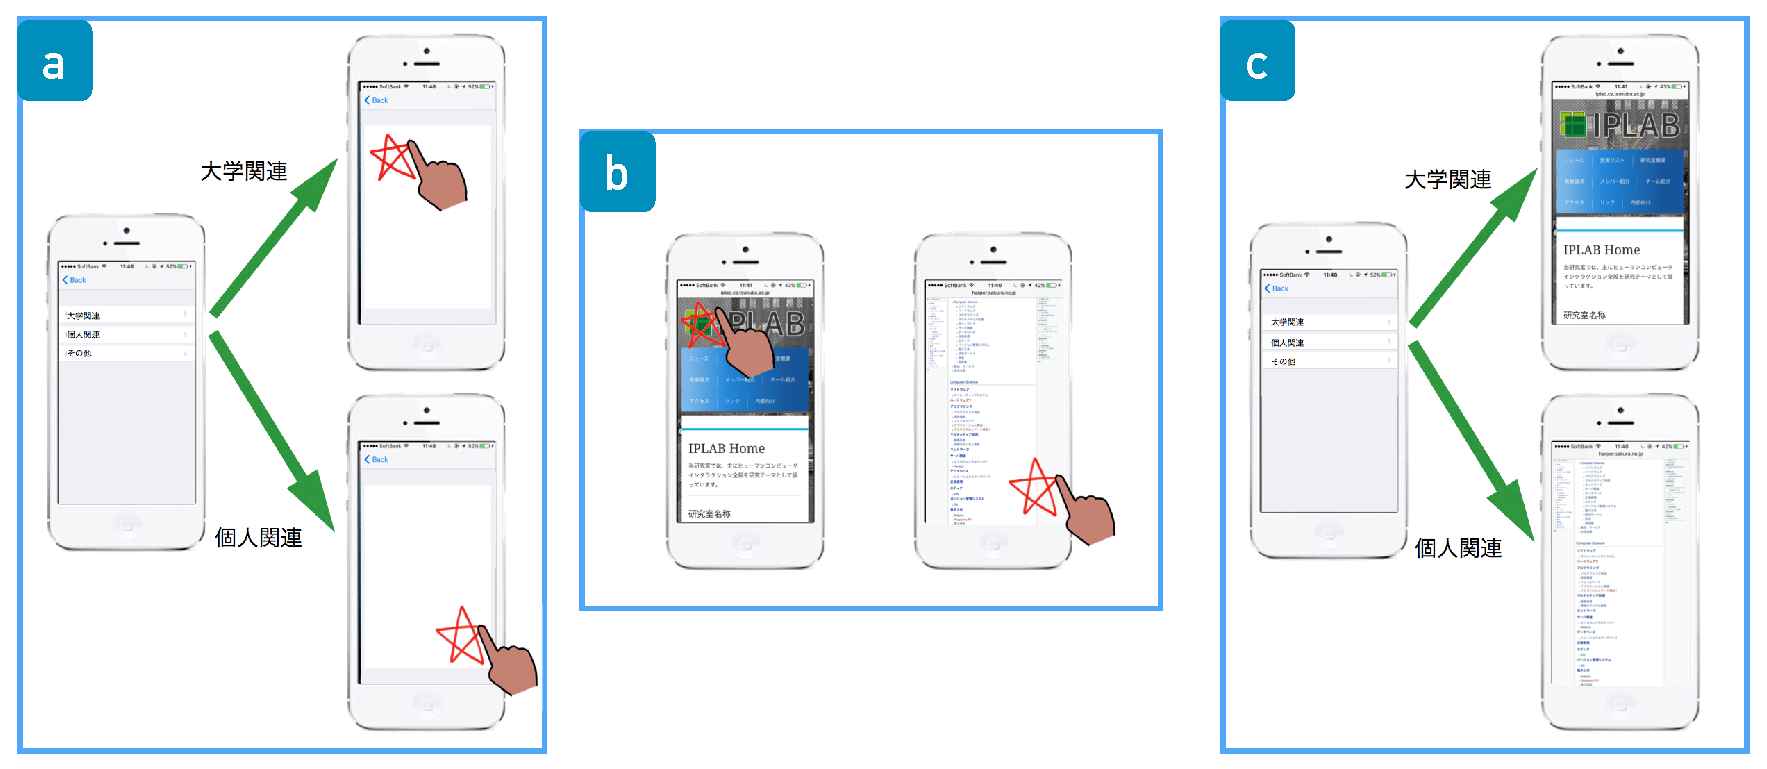
\includegraphics [width=1.0\hsize ]{img/phone_bookmark.eps}
	\end{center}
	\caption{ブラウザにおいて,手書きジェスチャによりブックマークの登録先を指定している例.(a)同じ書き順及び同じ形状であるが,位置の違いをブックマークの登録先に割り当てている.(b)webページ上にて,登録したいブックマークの種類に応じて,適当な位置に手書きジェスチャを入力すると,(c)ブックマークにそのwebページが登録される.}
	\label{fig:phone_bookmark}
\end{figure}

\clearpage
これらのアプリケーション例は,本研究における手書きジェスチャに関するユーザ調査において,被験者が考案した例である.
このようにして,アプリケーション内部に\$Vを実装することによって,同じ書き順及び同じ形状であるが,大きさ,向き,位置の違いを利用した手書きジェスチャの入力を用いたアプリケーションを開発することができる.この際,学習データは1つ追加するのみでよく,それぞれの手書きジェスチャが識別されるような重みが自動計算されている.


%このようにして,学習データを1つ追加するのみによって,手書きジェスチャを入力として用いるアプリケーションを開発できる.
同じ書き順及び同じ形状であるが,大きさ,向き,位置の違いを利用した手書きジェスチャを識別できると次のように手書きジェスチャを登録することができる.
例えば,同じカテゴリの操作に対しては,同じ書き順及び同じ形状の手書きジェスチャを用い,大きさ,向き,位置の違いを利用することによって,より実際の動作に即した手書きジェスチャを割り当てることが可能となる.これは,アプリケーションユーザにとって,登録した手書きジェスチャを覚えることが容易になるということにもつながる.
また,大きさ,向き,位置の違いを利用できない場合と比べて,利用可能な手書きジェスチャの種類が大きく拡大し,アプリケーションユーザが入力として用いたい手書きジェスチャを考案しやすくなったといえる.


